\section{Middlebox Design}
\label{sec:mb-design}

While it is possible to apply NetShaper framework's approach at any network layer, we chose to develop the system as an L4 (Transport Layer) proxy.
This enables the system to be easily deployable, entirely in userspace and without requiring any superuser privileges. 
Developing NetShaper at L2 (Data Link Layer) or L3 (Network Layer) would require the deployer to either have the ability to modify the OS kernel or deploy some form of kernel bypass.

\begin{figure}[!htb]
    \centering
    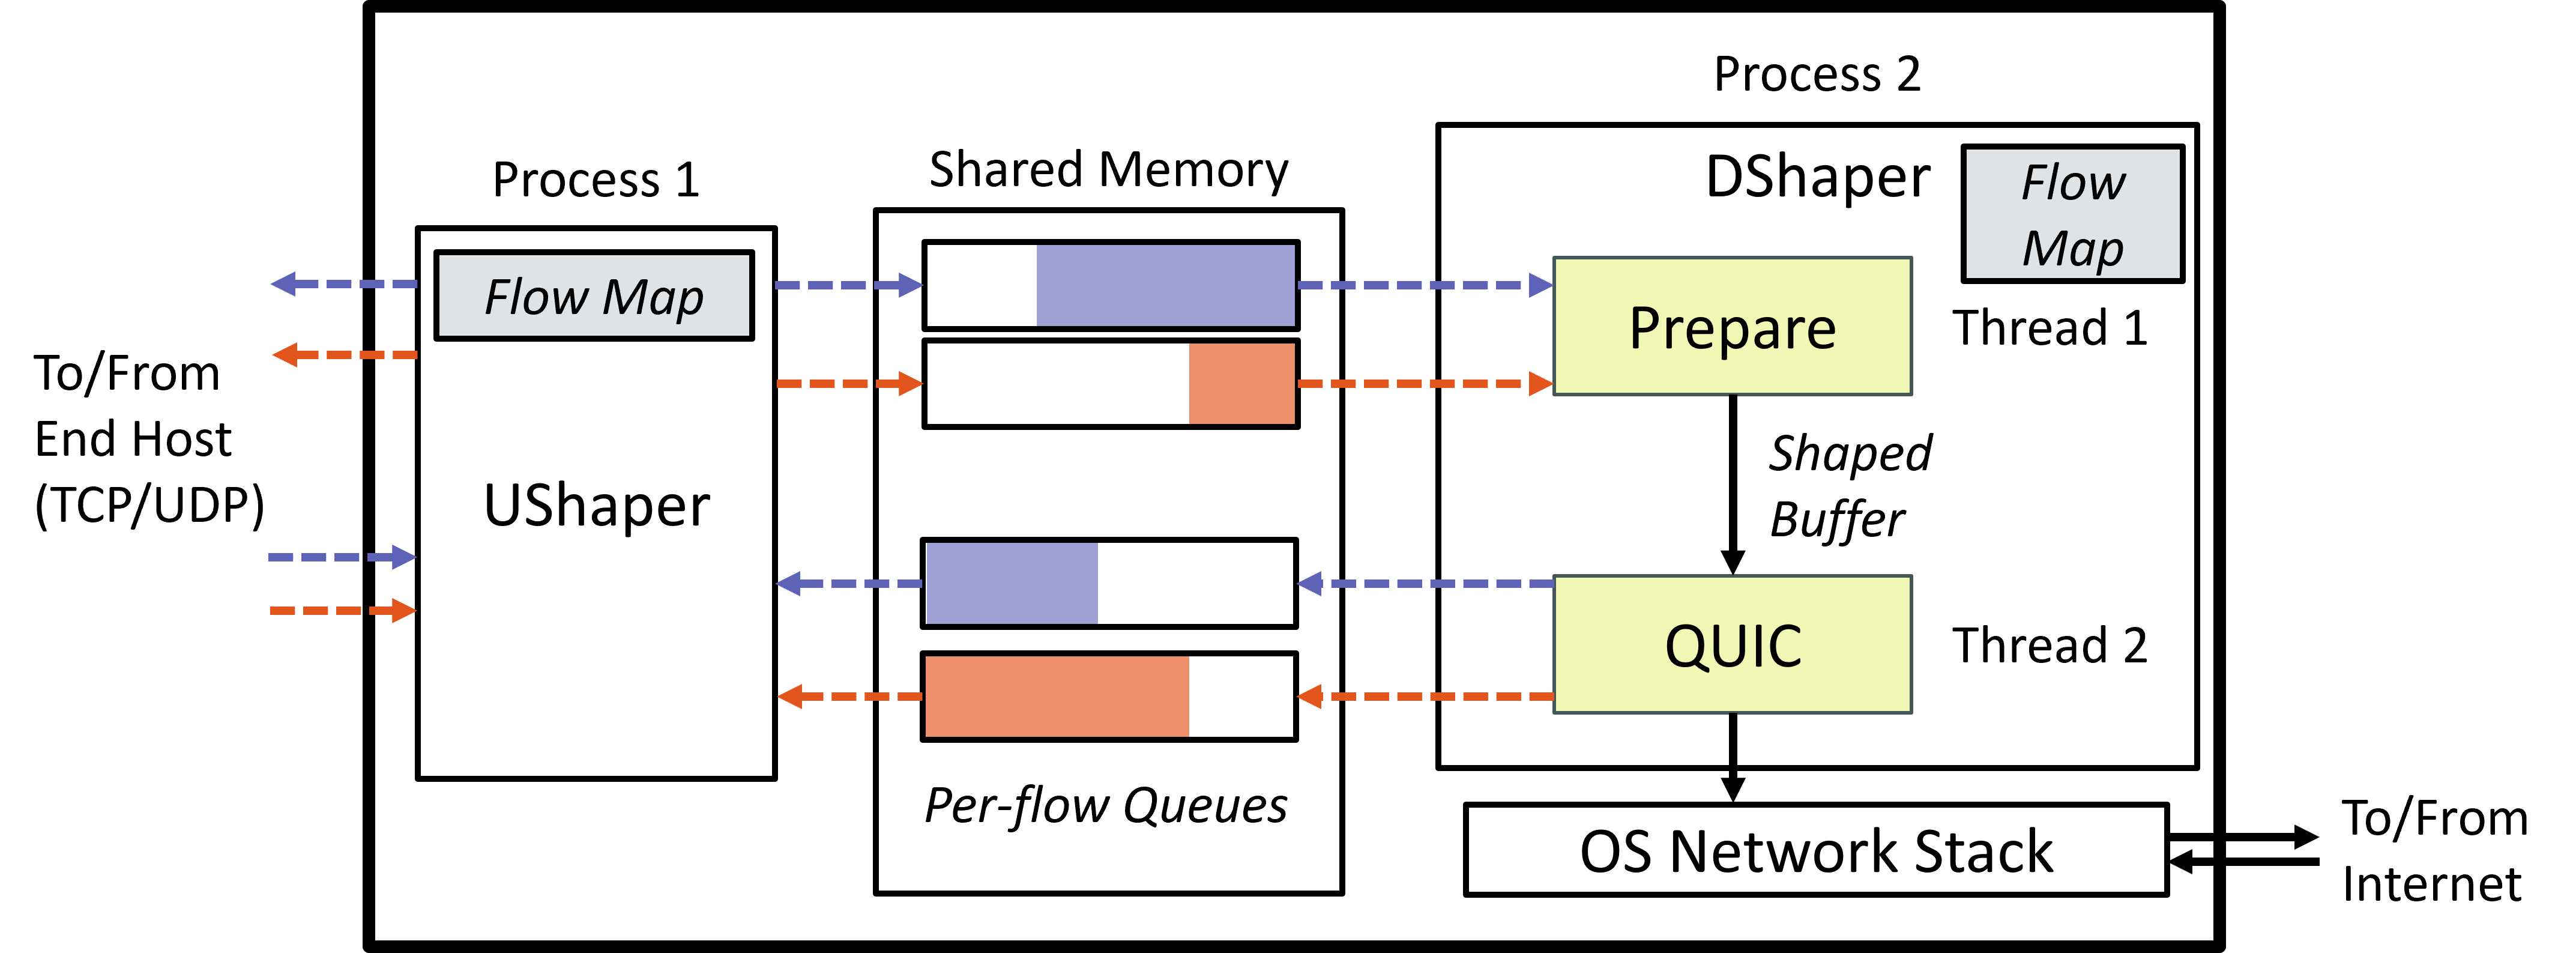
\includegraphics[width=\columnwidth]{figures/netshaper/middlebox-design.png}
    \caption{NetShaper Middlebox Design}
    \label{fig:middlebox-design}
\end{figure}

As outlined in \Cref{fig:middlebox-design}, NetShaper's middlebox consists of two main processes: UShaper and DShaper, and a shared memory between them.

\paragraph{UShaper.}
The \textit{UShaper} implements a client or a server to communicate with the end host.
It shares some Lamport Queues (LQs) [??] with DShaper.
It also consists of a flow map that maps a client with a corresponding pair of LQs.
\textit{UShaper} updates the flow map whenever a client establishes or terminates a connection.
In addition, it assigns an unused pair of LQs (one outbound and one inbound) to a new client and revokes that whenever the client terminates the connection.
The \textit{UShaper} receives outbound traffic from the end host and enqueues the payload in the assigned LQ.
Similarly, it dequeues inbound traffic from the inbound LQs and sends it to the corresponding end hosts.

\paragraph{DShaper.}
The \textit{DShaper} consists of two threads: \textit{Prepare} and \textit{QUIC worker}, and a flow map.
The flow map maps an LQ with a pre-initialised QUIC stream.
The \textit{Prepare} thread also measures the data available in the outbound LQs at the start of the window $W$.
It then adds noise to this available size based on the DP parameters.
Finally, it enqueues the payload and padding that needs to be transmitted.
The \textit{QUIC worker} transmits the enqueued data out to the network.
It also processes the received data, places it in the relevant LQ, and updates the flow map whenever a client initialises or terminates a connection.

In order to ensure that the operation of \textit{UShaper}, \textit{Prepare}, and \textit{QUIC worker} do not interfere with each other, we apply a few constraints in the implementation, and during the deployment of NetShaper.
First, all three components are required to be pinned on separate cores so that the execution time of one may not impact the others.
Second, in order to not leak the size of the payload due to the processing time of the enqueue operation done by the \textit{Prepare} thread, the \textit{Prepare} thread applies a lock for a fixed duration, during which the \textit{QUIC worker} can not transmit the data. 
We have outlined pseudo-code for both prepare and QUIC worker in \Cref{lst:prepare_and_worker}.
Finally, when receiving data, the \textit{QUIC worker} also enqueues the dummy bytes to a designated LQ so that the processing time remains consistent with the size of the data (see Figure ??).

\paragraph{Shared Memory.}
Both \textit{UShaper} and \textit{DShaper} have a shared memory between them.
This shared memory consists of three types of LQs: Control, Payload, Dummy
Similar to the stream types outlined in \Cref{sec:proxy-arch}, \textit{Control} LQ transmits the information about a connection establishment or termination by a client. 
\textit{Payload} LQ consists of the bytes received from the end host or to be sent to the end host.
\textit{Dummy} LQ consists of the dummy/padding bytes that are received.

\begin{minipage}{\textwidth}
\lstinputlisting[language=Python]{code/netshaper/prepare_and_worker.py}
\captionsetup{type=lstlisting}
\caption{Prepare and QUIC Worker Pseudo-code}
\label{lst:prepare_and_worker}
\end{minipage}

\endinput


\begin{figure}[!htb]
    \centering
    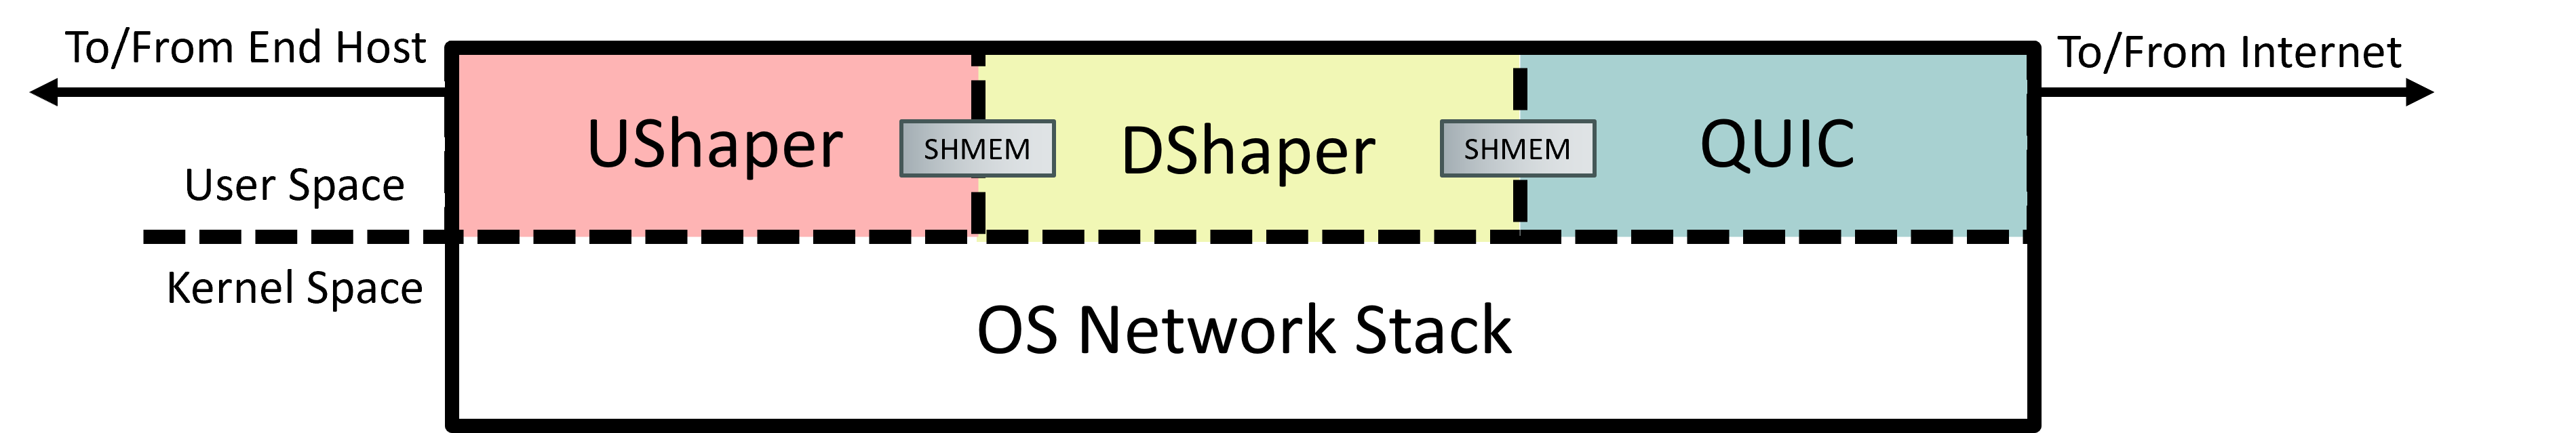
\includegraphics[width=\columnwidth]{figures/netshaper/middlebox-design-overview.png}
    \caption{Overview of NetShaper's Middlebox}
    \label{fig:middlebox-design-overview}
\end{figure}

\endinput

Should we add pseudo-codes for UShaper and DShaper?